\documentclass{article}
%----------------------------------------------------------------------
\usepackage[english]{babel}
\usepackage[utf8]{inputenc}
\usepackage[T1]{fontenc}
\usepackage[a4paper,top=2cm,bottom=2cm,left=3cm,right=3cm,marginparwidth=1.75cm]{geometry}
\usepackage{amsmath}
\usepackage{amsthm}
\usepackage{gensymb}
\usepackage{amssymb}
\usepackage{graphicx}
\usepackage[colorlinks=true, allcolors=black]{hyperref}
\usepackage{blindtext}
\usepackage{nomencl}
\usepackage{amsfonts}
\usepackage{listings}
\usepackage{xcolor}
\usepackage{float}
\usepackage{etoolbox}
\usepackage{tabularray}
\usepackage{array}
\usepackage{enumitem}
\usepackage{tikz}
\usetikzlibrary{graphs, graphs.standard}
%----------------------------------------------------------------------
\usepackage{algorithm}
\usepackage{algpseudocode}

\usepackage{csquotes}
\usepackage[backend=biber, style=numeric]{biblatex}
\addbibresource{refs.bib}

% ----------------------------------------------------

\begin{document}
	
	\begin{titlepage}
		\centering
		\vspace{1.5cm}
		
\includegraphics[width=0.9\textwidth]{WMiNI_logo.png} \\
		\vspace{1cm}
		{\fontsize{30}{20}\selectfont \textbf{CAD/CAM system design} \par}
		\vspace{1.5cm}
		{\fontsize{25}{20}\selectfont \textbf{Parametric Model of a Hexagonal Nut}\par}
		\vspace{1cm}
		{\fontsize{12}{20}\selectfont inż. Radosław Głasek\par}
		\vspace{1cm}
		{\fontsize{12}{20}\selectfont Supervisor: \\ mgr inż. Przemysław Zdroik \par}
		
		% \vfill
		% Oświadczam, że niniejsza praca, stanowiąca podstawę do uznania osiągnięcia efektów uczenia się z przedmiotu \textit{Projektowanie systemów CAD/CAM}, została wykonana samodzielnie. 
		
		\vspace{1cm}
		
		Warsaw, \today
		
	\end{titlepage}
	
	\newcommand{\ISONUTS}[0]{\textbf{ISO 4032:2012} }
	\newcommand{\ISOSYMBOLS}[0]{\textbf{ISO 225:2010} }
	\newcommand{\ISOMETRICSCREW}[0]{\textbf{ISO 68-1:1998} }
	
	%----------------------------------------------------------------------
	\tableofcontents
	\newpage
	
	%----------------------------------------------------------------------
	\section{Introduction}
	
	The subject of this project is a parametric model of a hexagonal
	nut. The description is based on \ISONUTS \cite{iso4032}, \ISOSYMBOLS \cite{iso225} and \ISOMETRICSCREW \cite{iso68}.
	
	The model was created in FreeCAD with all dimensions being driven by a spreadsheet, 
	enabling the nut to be easily reconfigured.
	
	% -------------------------------------------------------------------
	\section{Reference Standards}
	\begin{itemize}
		\item \ISONUTS --- Hexagon regular nuts (style 1) -- Product grades A and B
		\item \ISOSYMBOLS --- Fasteners -- Bolts, screws, studs and nuts -- Symbols and descriptions of dimensions
		\item \ISOMETRICSCREW --- ISO general purpose screw
		threads --- Basic profile --- Part~1. Metric screw threads
	\end{itemize}
	
	% -------------------------------------------------------------------
	\section{Parameters}
	The primary input is the metric thread designation (e.g. M10).
	Selecting a thread type populates a lookup table derived from \ISONUTS. Values for M10 thread are presented in table \ref{tab:defaults}. 
	After the thread type is selected, any individual parameter can be overridden.
	Thread profile dimensions computed from the pitch~$P$ are presented in table \ref{tab:thread}. 
	
	Angular parameters are set to values presented in table \ref{tab:angles}. 
	\begin{table}[ht]
		\centering
		\caption{Parameters and their default values for M10 thread type (dimensions in millimetres; nominal/max)}
		\label{tab:defaults}
		\begin{tblr}{
				colspec = {l c c c c},
				row{1} = {font=\bfseries},
				hline{1,2,Z} = {0.8pt},
			}
			Parameter & Symbol & M10 \\
			Basic major diameter (nominal diameter) of thread      & $D$   & 10    \\
			Pitch                 & $P$   & 1.5   \\
			% Washer face height    & $c$   & 0.60  \\
			Diameter of the countersink  & $d_a$ & 10.80 \\
			Outer diameter of the bearing face & $d_w$ & 14.60 \\
			Width across corners  & $e$   & 17.77 \\
			Nut height            & $m$   & 8.40  \\
			% Wrenching height      & $m_w$ & 6.40  \\
			Width across flats    & $s$   & 16.00 \\
		\end{tblr}
	\end{table}
	
	\begin{table}[ht]
		\centering
		\caption{Thread profile dimensions derived from pitch~$P$ (dimensions in millimetres)}
		\label{tab:thread}
		\begin{tblr}{
				colspec = {l l l},
				row{1} = {font=\bfseries},
				hline{1,2,Z} = {0.8pt},
			}
			Parameter & Formula & Value for M10 ($P=1.5$) \\
			Fundamental triangle height
			& $H = \frac{\sqrt{3}}{2}\,P$ & 1.299 \\
			Thread depth (nut)
			& $\frac{5}{8}\,H$ & 0.812 \\
			Crest truncation
			& $\frac{H}{8}$ & 0.162 \\
			Root truncation
			& $\frac{H}{4}$ & 0.325 \\
		\end{tblr}
	\end{table}
	
	\begin{table}[H]
		\centering
		\caption{Angular parameters.}
		\label{tab:angles}
		\begin{tblr}{
				colspec = {l l l},
				row{1} = {font=\bfseries},
				hline{1,2,Z} = {0.8pt},
			}
			Symbol & Description & Value \\
			$\theta$ & Countersink angle
			& $120\degree$ \\
			$\beta$  & External chamfer angle
			& $30\degree$ \\
			Thread flank angle & -- & $60\degree$ \\
		\end{tblr}
	\end{table}
	
	\section{Technical Drawing}
	Figure~\ref{fig:drawing} presents an annotated technical drawing of the
	hexagonal nut with the key dimensions labelled. 
	
	\begin{figure}[htbp]
		\centering
		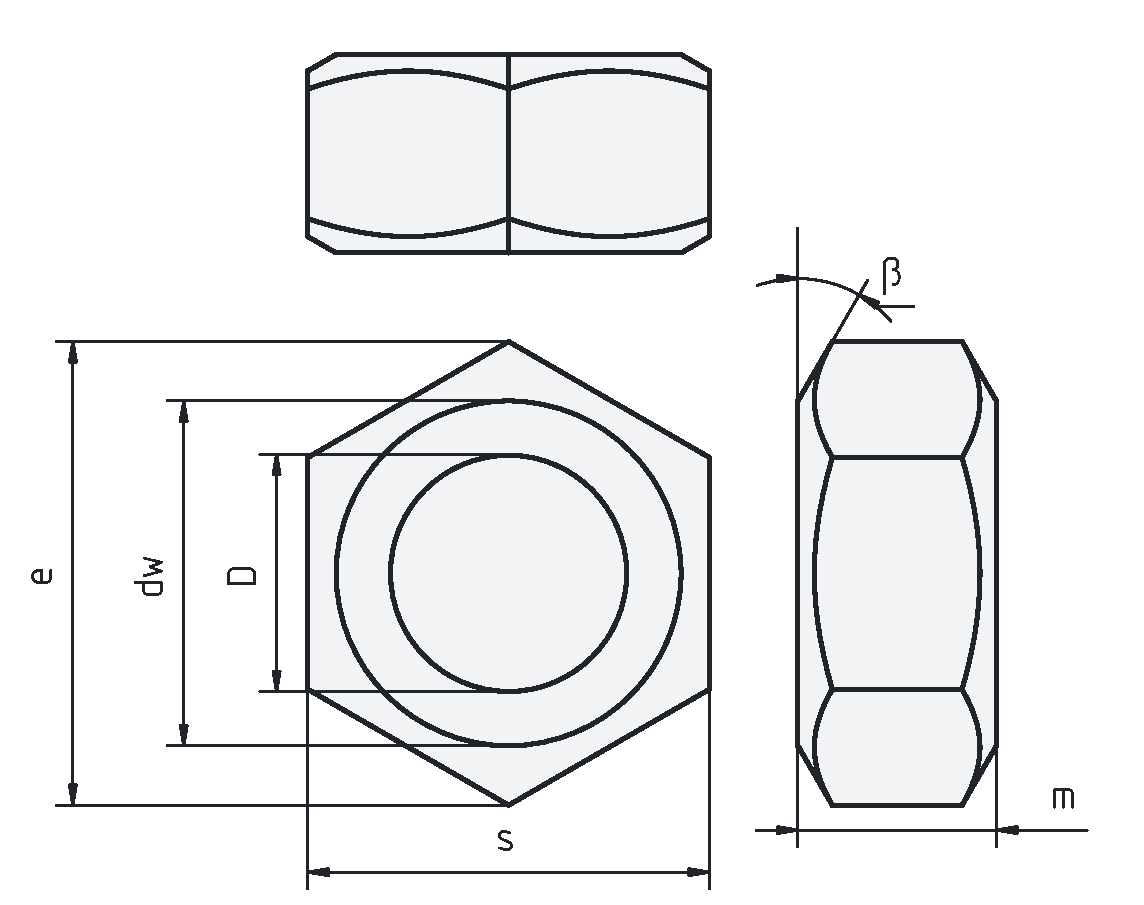
\includegraphics[width=0.75\textwidth]{proj.pdf}
		\caption{Technical drawing of the hexagonal nut with parameter annotations}
		\label{fig:drawing}
	\end{figure}
	
	\newpage
	\printbibliography
	
\end{document}